\chapter{Lecture 13 Least Squares Curve Fitting}
\label{ch:lec13n}
\section{Objectives}
The objectives of this lecture are to:
\begin{itemize}
\item Derive the basic formulas for least squares curve fitting.
\item Do an example using MATLAB.
\end{itemize}
\setcounter{lstannotation}{0}

\section{Introduction}
As an engineer, it is very likely that at some point in time during your career,
you will be called upon to examine and interpret experimental data.  Two
common needs in such analysis are to take a set of experimental data and either:
\begin{enumerate}[label=\alph*.)]
\item develop a model to represent the data. i.e. find a best fit line (or
  other function) through
  the data; or
\item evaluate the data to determine how well it agrees with some previously
  defined model.  i.e. fit model parameters to the data and assess how well
  the experimentally determined values conform to model expectations.

\end{enumerate}

As an example, we will perform a data-fitting analysis of some wind-tunnel
results as presented in popular numerical methods textbook.\cite[-1.5cm]{gilat} The behavior that we will explore is the dissipation of vortices shed from the tips and trailing
edges of an airfoil in the wind tunnel.  For this example, the tangential
velocity $\left(V_{\theta}\right)$ of a vortex is measured as it travels down the axis of a
wind-tunnel.  The data is non-dimensionalized by dividing the tangential
velocity of the vortex by the free-stream velocity $\left(V_{\infty}\right)$ and by dividing the vortex
position $\left(R\right)$ relative to the airfoil by the chord-length $\left(C\right)$ of the airfoil.  This non-dimensionalization process will allow experimenters to correlate the results from one particular experiment to larger scale tests on geometrically similar prototypes.  The raw data is given in Table \ref{tab:lec13n-numData} and is shown graphically in Figure \ref{fig:lec13n-theData}.
\begin{marginfigure}[-2.5cm]
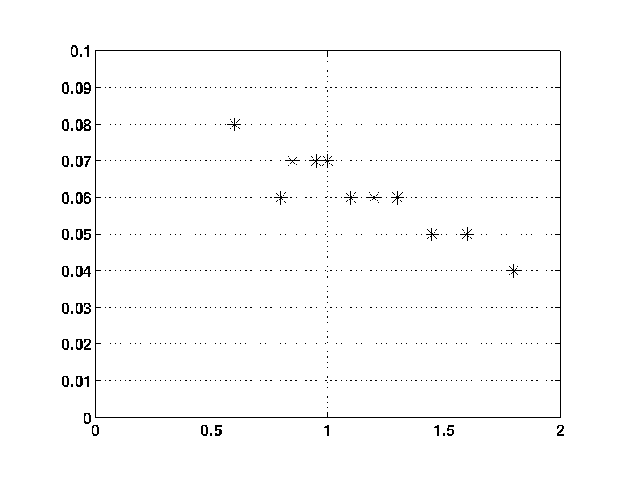
\includegraphics{lec13n_TheData.eps}
\caption{Experimental data from wind tunnel testing.  The $y$-axis is the
  ratio of the tangential velocity of a vortex to the free stream flow
  velocity $\left( y = \sfrac{V_{\theta}}{V_{\infty}}\right)$.  The $x$-axis is
  the ratio of the distance from the vortex core to the chord of an aircraft
  wing. $\left(x = \sfrac{R}{C}\right)$.}
\label{fig:lec13n-theData}
\end{marginfigure}
\begin{table}[h]
\centering
\begin{tabular}{|l|*{11}{c}|}
\hline
$x = \sfrac{V_{\theta}}{V_{\infty}}$ & 0.6 & 0.8 & 0.85 & 0.95 & 1.0 & 1.1 &
  1.2 & 1.3 & 1.45 & 1.6 & 1.8 \\
\hline
$y = \sfrac{R}{C}$ & 0.08 & 0.06 & 0.07 & 0.07 & 0.07 & 0.06 & 0.06 & 0.06 & 0.05 &
  0.05 & 0.04 \\
\hline
\end{tabular}
\caption[][1.5cm]{Numerical data from wind-tunnel experiment.}
\label{tab:lec13n-numData}
\end{table}
In the following sections, we will explore ways in which curves can be fit through this data which, in some sense, are the ``best''-fit curves.

\section{``Guessed''-fit Curves}
It is entirely reasonable, and completely in accord with time honored engineering tradition, to take experimental data as presented in the previous section, use careful judgment and intuition and draw a line that seems to fit the data reasonably well. We will call this the \emph{Guessed}-fit curve and an example of this is shown in Figure \ref{fig:lec13n-guessedfit}.

\begin{marginfigure}
\includegraphics{GuessedFit.eps}
\caption{\emph{Guessed}-fit linear estimation of the experimental data.  $M =
  -0.033$ is the measured slope of the estimated line and $b = 0.1$ is the $y$-intercept.}
\label{fig:lec13n-guessedfit}
\end{marginfigure}  

From this carefully drawn line we may conclude that experimental results show a linear
relationship between tangential velocity and distance downstream from the
airfoil.  Obviously, this model is not perfect; most data-points are off the
line.  Still, we may reasonably decide that overall, this is not a bad
representation of what the data are telling us and leave well enough alone.

\section{Measure of Fitness}

A hand-drawn curve may be well enough for rough analysis, but for the purposes of this primer, let us assume that we would like to know how good our roughly drawn curve is and wonder if there may be a way to do better.  We have a good fit; but how good is it?  In this section we will answer that question.  We will define a \emph{measure of fitness} so that we may quantitatively determine how ``good'' a candidate curve is in representing the data.

 
For this purpose, we define the \emph{residual}.  In words, the residual $(r_i)$ is the
difference, at each experimental data point $(x_i)$, between the $y$-value given from experimental data $(y_i)$ and the $y$-value computed from our linear ``guessed'' fit curve $\left(y_{\text{guessed}}\right)$.  The mathematical expression for this is given in Equation \ref{resid}.

\begin{equation}
r_{i} = y_{i} - \underbrace{\left(b + Mx_{i}\right)}_{y_{\text{guessed}}} \ \ i = 1,2,\dots,n
\label{resid}
\end{equation}
where $b$ is the $y$-intercept of this linear fit and $M$ is the slope of
the linear fit through the data
and $n$ is the number of data points.

With an eye towards a more general approach, we will re-state Equation \ref{resid} using matrix-vector notation in Equation \ref{residV2}.

\begin{equation}
\begin{split}
\mathbf{r} &= \mathbf{y} - \underbrace{\left( b \cdot \mathbf{x}^0 + M \cdot
\mathbf{x}^{1}\right)}_{\mathbf{y}_{\text{guessed}}} \\
 &= \mathbf{y} - 
\left[
\begin{matrix}
\mathbf{x}^{0} & \mathbf{x}^{1}
\end{matrix}
\right]
\left[
\begin{matrix}
b \\
M
\end{matrix}
\right] \\
&= \mathbf{y} - \mathbf{X}\mathbf{c}
\end{split}
\label{residV2}
\end{equation}

To be clear, please note that $x^{k}$ refers to element-wise exponentiation and in particular, $\mathbf{x}^{0}$ means: ``each element of $\mathbf{x}$ raised to the power of zero,'' and $\mathbf{x}^{1}$ means: ``each element of $\mathbf{x}$ raised to the first power.''  

In order to determine how well a given curve fits the data, the residual given in Equation \ref{residV2} is not quite satisfactory; it is a vector, not a number.  The usual solution to this problem is to use the Euclidean length of the residual as shown in Equation \ref{norm2Resid}:

\begin{equation}
\begin{split}
||r|| &= \sqrt{\mathbf{r}^{T} \mathbf{r}} \\
 &= \sqrt{\sum_{i=1}^{n} r_{i} \cdot r_{i}} 
\end{split} 
\label{norm2Resid}
\end{equation}

For historical reasons, we will depart from this convention and use the ``Euclidean length squared,'' or simply the square of the residual.  We show this in Equation \ref{residSquared} where we also explicitly expand $\mathbf{r}$ as defined in Equation \ref{residV2} to show the residual in terms of the given data $\mathbf{y}$, the matrix $\mathbf{X}$ of our fitting curve and parameter vector $\mathbf{c}$.

\begin{equation}
\begin{split}
\mathbf{r}^{2} &= \mathbf{r}^{T} \mathbf{r} \\
 &= \left(\mathbf{y} - \mathbf{X}\mathbf{c}\right)^{T}\left(\mathbf{y} -
\mathbf{X}\mathbf{c}\right) \\
&= \mathbf{y}^{T}\mathbf{y} - 2 \mathbf{c}^{T}\mathbf{X}^{T}\mathbf{y} +
\mathbf{c}^{T}\mathbf{X}^{T}\mathbf{X}\mathbf{c} 
\end{split}
\label{residSquared}
\end{equation}

The error measure given in Equation \ref{residSquared} now is a single
non-negative number that will in general be zero only if the fitted line passes exactly through all data points.  This is the measure of fitness that we will use.
Using the given values of $\mathbf{y}$, $\mathbf{X}$ and $\mathbf{c}$ for the
``guessed''-fit curve, we find that $\left(\mathbf{r_{\text{guessed}}}\right)^{2} = 0.0152.$ 

\section{Method of Least Squares}

So far we have naively attempted to fit the data as best as we can by guessing
a linear function that might in some way represent the data.  We have defined
an error measure that confirms our suspicion that our linear curve fit is not
perfect.  It is natural to wonder: is there a line that \emph{best} fits the
data\sidenote{At least ``best'' by some error measure.  Different error measures sometimes yield different answers as to what constitutes ``the best.''} and if so, how do we find it? The answer is \emph{``yes, there is a way to find the best fit line''} and the method to find it is called the method of least squares. 

\subsection{Algebraic Derivation}

The standard algebraic derivation of the method of least squares starts with the squared residual given in Equation \ref{residSquared}.  As you should take a moment to confirm, once we have selected a linear estimator\sidenote{
i.e. we have chosen what functions will be used to make up the columns of
$\mathbf{X}$---for the time being we decided it would be composed of the 0th
and 1st powers of $\mathbf{x}$} $\mathbf{X}$, the only free parameter in Equation
\ref{residSquared} are the coefficients that make up $\mathbf{c}$.  The goal
is to figure out how to choose $\mathbf{c}$ such that the error given in
Equation \ref{residSquared} is as small as possible.

Recall from your introductory calculus courses that the way to minimize a
function is to take the first and second derivative of the function; solve for
the values of the free parameter $(\mathbf{c})$ so that the first derivative
is equal to zero; and verify that the second derivative is positive.  When the
first derivative is zero, the function is at an extrema; when the second
derivative is positive, that extrema is a minimum.

Carrying out this idea, we will take the derivative of Equation
\ref{residSquared} and set the first derivative equal to zero:

\begin{equation}
\begin{split}
\frac{d}{d\mathbf{c}}\mathbf{r}^{2} = 0  - 2\mathbf{X}^{T}\mathbf{y} + \underbrace{\mathbf{X}^{T}\mathbf{X}\mathbf{c} + \mathbf{c}^{T}\mathbf{X}^{T}\mathbf{X}}_{\mathbf{X}^{T}\mathbf{X}\mathbf{c} = \mathbf{c}^{T}\mathbf{X}^{T}\mathbf{X}} &= 2\left(-\mathbf{X}^{T}\mathbf{y}+
\mathbf{X}^{T}\mathbf{X} \mathbf{c}\right) = 0 \\
&\Rightarrow -\mathbf{X}^{T}\mathbf{y} + \mathbf{X}^{T}\mathbf{X}\mathbf{c} =
0 \\
&\Rightarrow \mathbf{X}^{T}\mathbf{X} \mathbf{c} = \mathbf{X}^{T}\mathbf{y}
\end{split}
\label{normalEq}
\end{equation}

We now have to ask: can we find a unique vector $\mathbf{c}$ such that the
last line in Equation \ref{normalEq} is satisfied?  The answer is:
yes---provided only that the columns of $\mathbf{X}$ are linearly
independent\sidenote{If the columns of $\mathbf{X}$ are linearly independent, this means---by definition---that $\mathbf{Xy} = 0$ if and only if $\mathbf{y}=0$.}, $\mathbf{X}^{T}\mathbf{X}$ will be positive-definite and thus non-singular\sidenote{When a matrix---$\mathbf{A} =
  \mathbf{X}^{T}\mathbf{X}$--- is positive definite, that means that
  $\mathbf{y}^{T}\mathbf{Ay}=0$ if and only if $\mathbf{y}=0$.  So $\mathbf{y}
  \ne 0$ and if the columns of $\mathbf{X}$ are linearly independent ($\mathbf{Xy} \ne 0$),
  then $\mathbf{y}^{T}\mathbf{X}^{T}\mathbf{X}^{T}\mathbf{y} \ge 0$ and can
  \emph{only} be equal to zero if $\mathbf{y}=0$.  As is discussed in
  in previous lectures, positive-definiteness is a sufficient condition for a solution to Equation
  \ref{normalEq} to exist.}.  This means that a unique value of $\mathbf{c}$
will exist and that it will be non-zero:

\begin{equation}
\mathbf{c} = \left(\mathbf{X}^{T}\mathbf{X}\right)^{-1}
\left(\mathbf{X}^{T}\mathbf{y}\right)
\label{lstSqSol}
\end{equation} 


MATLAB code to carry out this process is given below:

\begin{lstlisting}[style=myMatlab]
x = [0.6 0.8 0.85 0.95 1.0 1.1 1.2 1.3 1.45 1.6 1.8]; 
y = [0.08 0.06 0.07 0.07 0.07 0.06 0.06 0.06 0.05 0.05 0.04]; 

X = nan(length(x),2);
X(:,1) = (x').^0;
X(:,2) = (x').^1;

c = (X'*X) \ (X'*y');
\end{lstlisting}
